\documentclass[a4paper,oneside,12pt]{article}

\usepackage{standalone}

\usepackage{vhistory}
\usepackage{setspace}
\usepackage[numbers]{natbib}
\usepackage{url}
\usepackage[utf8]{inputenc} 
\usepackage[english,danish]{babel} 
\usepackage{lmodern} % Modern LaTeX font
\renewcommand{\danishhyphenmins}{22} 
\usepackage[T1]{fontenc}
\usepackage{amsmath,amssymb,bm,mathtools}
\usepackage{gensymb}
\usepackage[load-configurations=version-1]{siunitx}
\usepackage{graphicx}
\usepackage{svg}
\usepackage{float}
\usepackage{setspace}
\usepackage[font=footnotesize]{caption}
\usepackage{fancyhdr}
\pagestyle{fancy}


\begin{document}
\begin{titlepage}
\centering
\vfill
{\LARGE Kravspecifikation}\\
\vfill
{\bfseries\large
	Bachelorprojektet: \\
	Real-time eye-tracking\\
	Projektnummer: 15017\\
}
\vfill

\includegraphics{ASE_logo.png}
\vfill
{\bfseries\large
	Version 1.1\
	30/01/2015\\
	Studerende: Søren Vøgg Krabbe Lyster (SVL) 10920,\\
	Martin Degn Kristensen (MDK) 10441\\ 
	Studieretning: Elektro \\
	Vejleder: Preben Kidmose \\
	\vfill	
	\rule{6cm}{1pt}
}




\end{titlepage}
\lhead{
\includegraphics[scale=0.2]{ASE_logo.png}}
\chead{Real-time eye-tracking}
\rhead{\scriptsize 30/01/15 \\
S. V. K. Lyster, M. D. Kristensen}
\begin{versionhistory}
	\vhEntry{1.0}{26.01.15}{SVL,MDK}{Oprettet}
	\vhEntry{1.1}{30.01.15}{SVL,MDK}{Opdateret m. use cases}
\end{versionhistory}
\tableofcontents
\documentclass[accepttest.tex]{subfiles}
\begin{document}
	\section{Indledning}
	\subsection{Formål}
	 Formålet med accepttesten er at opstille en række tests, specifikt udarbejdet til at verificere om de krav
	 der bliver fremvist i kravspecifikationen bliver opfyldt af produktet/prototypen. Dette gør det lettere hurtigt
	 at se om en given version af produktet/prototypen er tilfredsstillende.
	 \subsection{Referencer}
	  Accepttesten er opbygget ud fra de krav der er stillet af projektudbyderen (Preben Kidmose), samt
	  krav der løbende er opstået igennem udviklingen af produktet/prototypen. Disse krav er specificeret i dokumentet Kravspecifikation.
	  \subsection{Omfang og begrænsninger}
	  Accepttesten inderholder test af det samlede produkt og er den endelige
	  afprøvning af produktet.
	  \subsection{Godkendelseskriterier}
	  Accepttesten er afsluttet, når alle specificerede test cases er gennemført og godkendt.
	  Hvis der under accepttesten opstår fejl, der umuliggør fortsat udførsel af de efterfølgende test cases,
	  afbrydes accepttesten.
	  
	  Hvis der opstår fejl i enkelte test cases; men fortsat accepttest er mulig, underkendes den enkelte test og
	  accepttesten fortsætter med de næste test cases.
	  
	  Såfremt en test afbrydes eller en test case underkendes, skal der udfærdiges en problemrapport, der beskriver
	  årsagen til underkendelsen. Problemrapporten skal efterfølgende godkendes af både kunde og leverandør.

\subsection{Læsevejledning}
Dette dokument er bygget op af en række test-cases. Disse test-cases har til formål at verificere alle krav stillet i projektets kravspecifikation. De forskellige tests er bygget op med vejledning om hvordan de foretages. \textit{Forberedelse} beskriver hvordan systemet skal gøres klart før brug. \textit{Aktion} beskriver de handlinger der skal foretages for at udføre testen. \textit{Forventet resultat} beskriver det forventede resultat af testen. \textit{Accepteret} er til at notere om test-casen er godkendt eller afvist. 

Afsnittet performanceevaluering har til formål at teste systemets performance. Dette afsnit er ikke tilknyttet kravspecifikationen, da det ikke er bygget på krav fra projektudbyderen.
	  \pagebreak
\subsection{Test-rutiner}
Følgende rutiner beskrevet her vil blive refereret senere i accepttesten.
\subsubsection{Tal-test}
\label{taltest}
\begin{figure}
\centering
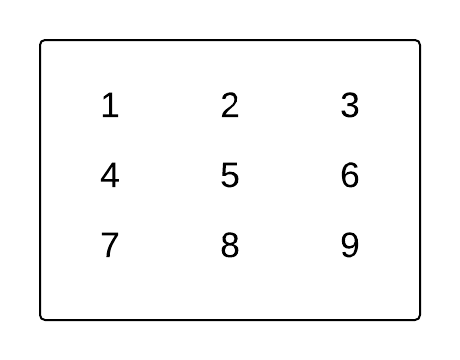
\includegraphics[width=0.5\linewidth]{Tal-test}
\caption{Layout af grafik på skærm for tal-testen.}
\label{fig:Tal-test}
\end{figure}
I denne test bliver testpersonen bedt om at fokusere på tallene i en bestemt rækkefølge. For eksempel $ 1,9,7,6,8,3\ldots $ Rækkefølgen bestemmes af brugeren. Herved kan den samme test gengives flere gange ved at genbruge samme talrække.

%\subsubsection{Krydsvalidering}
%$ DS 1 \rightarrow KAL 1 \rightarrow XY $ \hspace{2cm}
%$ DS 2 \rightarrow KAL 2 \rightarrow XY $ \\
%$ DS 1 \rightarrow KAL 2 \rightarrow XY $ \hspace{2cm}
%$ DS 2 \rightarrow KAL 1 \rightarrow XY $ \\
	  
\subsubsection{Dynamisk test}	  
\label{dyntest}
\begin{figure}
\centering
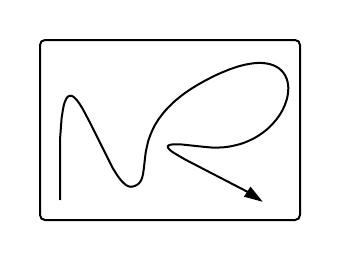
\includegraphics[width=0.4\linewidth]{DynamiskTest}
\caption{Eksempel på sti der skal følges ved dynamisk test.}
\label{fig:DynamiskTest}
\end{figure}
Ved dynamisk test bedes testpersonen om at følge en linje der bliver tegnet på skærmen. Denne test har til formål at vise hvor godt systemet kan foretage eye-tracking ved konstant bevægelse. 

\end{document}
\documentclass[kravspec.tex]{subfiles}
\begin{document}
\section{Generel beskrivelse}
Dette afsnit i kravspecifikationen vil give et overodnet billede af de krav der er blevet opstillet for udviklingen af systemet.
	
\subsection{Systembeskrivelse}
\begin{figure}[h]
\centering
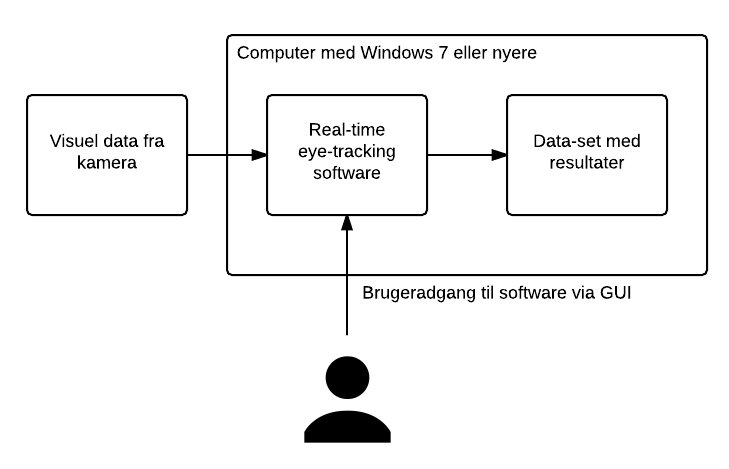
\includegraphics[width=0.7\linewidth]{Systemdiagram}
\caption[Systemdiagram]{Systemdiagram for Real-time eye-tracking}
\label{fig:Systemdiagram}
\end{figure}
Der ønskes udviklet et system som kan indsamle videodata fra et kamera og derefter anvende dataen til
at bestemme hvor en forsøgsperson kigger hen på en specifik skærm. Systemet skal derudover videregive
denne information til brugeren via koordinater samt en graf der repræsenterer den skærm forsøgspersonen
ser på.
\\
Før dataopsamling skal en indledende kalibrering af systemet gennemføres. Dette gøres ved at et gitter med
specifikke punkter indlæses på forsøgspersonsskærmen. Derefter bedes forsøgspersonen se på specifikke punkter
på skærmen, og sammenhængen imellem de målte punkter og de kendte punkter kan anvendes til at finde en
homografisk mapning. Efter denne kalibrering kan systemet anvendes.
\\
Systemet udvikles med henblik på en standard anvendelsesmåde, med mulighed for brugerdefinerede anvendelses-
måder. Standardanvendelsen omhandler at vælge en sti og et filnavn, hvorefter dataopsamling umiddelbart begynder.
Under dataopsamlingen vil gazevectoren løbende blive præsenteret for brugeren på brugerskærmen. Når brugeren er 
færdig kan opsamlingen stoppes, og dataopsamlingen gemmes i den tidligere valgte fil. Bemærk at den algoritme
der anvendes til behandling af data her er forudbestemt.
\\
(Hvis brugeren ønsker at bruge en anden algoritme kan denne indlæses. Den kan også indskrives direkte i
GUI'en, og derefter gemmes. Formålet med dette er at kunne indrette systemet efter specifikke behov, og
hurtigt indhente de opsætninger til fremtidig brug. Eventuelt kan andre variabler indtastes ved systemstart) 
\\
I de følgende afsnit fremgår det hvorledes det udviklede system indgår i det samlede system.


\subsection{Aktører}
En række af de kommende funktionelle krav vil blive opstillet som use-cases. Følgende er beskrivelser for de enkelte aktører: \\
\\
\begin{tabular}{| l | p{10cm} |}
	\hline 
	Navn & Bruger \\ \hline
	Beskrivelse & Brugeren er personen der tilgår systemet via et grafisk user interface.\\ \hline
\end{tabular}
\\ \\
\begin{tabular}{| l | p{10cm} |}
	\hline 
	Navn & Kamera \\ \hline
	Beskrivelse & Systemet vil snakke sammen med et kamera, hvis formål er at levere visuelt data.\\ \hline
\end{tabular}
\end{document}
\documentclass[accepttest.tex]{subfiles}
\begin{document}
	\section{Funktionelle krav}
Systemet testes med kamera, afstand og skærm som angivet i kravspecifikation punkt 4.
\subsection{Real-time eye-tracking}
\begin{table}[H]
	\small
\begin{tabular}{|p{3.5cm}|p{3.5cm}|p{3.5cm}|l|}
	\hline Forberedelse & Aktion & Forventet resultat & Accepteret \\ 
	\hline Computerprogrammet startes. Kameraet tilsluttes og tændes. Session oprettes. & Ny måling igangsættes. Efter ca. 10 sekunder stoppes testen. Den reelle tid af målingen kan aflæses i GUI. & Antal XY koordinater i log-filen skal stemme overens med tid af måling i sekunder $ \times $ 100 (framerate). &  \\ 
	\hline 
\end{tabular} 
\end{table}

\begin{table}[H]
	\small
\subsection{Kalibrering}
\begin{tabular}{|p{3.5cm}|p{3.5cm}|p{3.5cm}|l|}
	\hline Forberedelse & Aktion & Forventet resultat & Accepteret \\ 
	\hline Computerprogrammet startes. Kameraet tændes. Session oprettes. Et test-sæt af kalibreringsdata med høj afvigelse findes. En testperson skal bruges til kalibrering.  & 
	Tal-testen \ref{taltest} foretages med test-sættet af kalibreringsdata. Afvigelsen noteres. Ny kalibrering foretages. Tal-testen foretages igen. Afvigelsen noteres. & 
	Afvigelsen ved ny kalibrering er mindre end ved brug af test-sættet.  &  \\ 
	\hline 
\end{tabular} 
\end{table}

\subsection{Output}
\begin{table}[H]
	\small
\begin{tabular}{|p{3.5cm}|p{3.5cm}|p{3.5cm}|l|}
	\hline Forberedelse & Aktion & Forventet resultat & Accepteret \\ 
	\hline Måling foretages. & Efter måling tilgår brugeren log-filen. & Log-filen åbnes. Log-filen overholder protokollen. &  \\ 
	\hline 
\end{tabular} 
\end{table}

\subsection{Brugertilgang}
\subsubsection{Use case 1: Opret session}

\begin{table}[H]
	\small
\begin{tabular}{|p{2cm}|p{3cm}|p{3cm}|p{3cm}|l|}
	\hline Test case & Forberedelse & Aktion & Forventet resultat & Accept \\ 
	\hline Normal forløb & Computer-programmet startes.  Kameraet tilsluttes og tændes.  & Bruger klikker på ”Create session” og følger programmets anmodninger. & Bruger bliver returneret til menuen med beskeden ”Session created”. Der findes data- og opsætnings-fil i den angivne fil-sti. &  \\ 
	\hline 
\end{tabular} 
\end{table}

\subsubsection{Use case 2: Kalibrering}
\begin{table}[H]
	\small
\begin{tabular}{|p{2cm}|p{3cm}|p{3cm}|p{3cm}|l|}
	\hline Test case & Forberedelse & Aktion & Forventet resultat & Accept \\ 
	\hline Normal forløb & Computer-programmet er startet. Kameraet er tilsluttet og tændt. 
	Gyldig session oprettes. & Bruger klikker på ”Calibration”, derefter ”Continue” og følger så programmets anmodninger. & Bruger bliver returneret til menuen med beskeden ”Calibration complete”. Der findes data- og opsætnings-fil i den angivne fil-sti. & \\
	
	\hline Undtagelses-forløb 1 & Computer-programmet er startet. Kameraet er tilsluttet og tændt. Der er ikke oprettet en session. & Bruger klikker på ”Calibration”. & Bruger bliver informeret om at der ikke findes en gyldig session. Bruger bliver returneret til menu. &\\
	\hline Undtagelses-forløb 2 & Computer-programmet er startet. Kameraet er tilsluttet og tændt. 
	Gyldig session oprettes. & Bruger klikker på ”Calibration”, derefter ”Cancel”. & Bruger bliver returneret til menu. & \\
		\hline 
\end{tabular}
\end{table}

\subsubsection{Use case 3: Start måling}
\begin{table}[H]
	\small
	\begin{tabular}{|p{2cm}|p{3cm}|p{3cm}|p{3cm}|l|}
		\hline Test case & Forberedelse & Aktion & Forventet resultat & Accept \\ 
		\hline Normal forløb & Gyldig session er oprettet. Kalibrering er udført.  & Bruger klikker på ”Start”.   & Programmet starter en måling. Programmet viser at en måling er i gang. & \\
		
		\hline Undtagelses-forløb 1 & Gyldig session er oprettet. Kalibrering er ikke udført. & Bruger klikker på ”Start” & Programmet informerer bruger at kalibrering ikke er foretaget.  &\\
		\hline 
	\end{tabular}
\end{table}

\subsubsection{Use case 4: Stop måling}
\begin{table}[H]
	\small
	\begin{tabular}{|p{2cm}|p{3cm}|p{3cm}|p{3cm}|l|}
		\hline Test case & Forberedelse & Aktion & Forventet resultat & Accept \\ 
		\hline Normal forløb & Real-time eye-tracking måling igangsættes. & Bruger klikker på ”Stop” & Programmet stopper måling. Programmet viser at målingen er stoppet.  & \\
		\hline 
	\end{tabular}
\end{table}

\subsubsection{Use case 5: Gem indstillinger}
\begin{table}[H]
	\small
	\begin{tabular}{|p{2cm}|p{3cm}|p{3cm}|p{3cm}|l|}
		\hline Test case & Forberedelse & Aktion & Forventet resultat & Accept \\ 
		\hline Normal forløb & Programmet startes. & Bruger klikker på ”Save preferences”. Derefter vælges der filnavn og placering af fil. & Fil er oprettet i den valgte fil-sti. Fil indeholder de korrekte indstillinger. & \\
		
		\hline Undtagelses-forløb 1 & Programmet startes. & Bruger klikker på ”Save preferences”. Derefter vælges der ugyldig filnavn og fil-sti. & Programmet alarmerer at filen ikke kunne oprettes. Bruger bliver returneret til menuen. &\\
		\hline 
	\end{tabular}
\end{table}

\subsubsection{Use case 6: Indlæs indstillinger}
\begin{table}[H]
	\small
	\begin{tabular}{|p{2cm}|p{3cm}|p{3cm}|p{3cm}|l|}
		\hline Test case & Forberedelse & Aktion & Forventet resultat & Accept \\ 
		\hline Normal forløb & Programmet startes. En gyldig fil med indstillinger oprettes.  & Bruger klikker på ”Load preferences”. Derefter vælges gyldig fil med  indstillinger. & Programmet har samme indstillinger som angivet i filen.  & \\
		
		\hline Undtagelses-forløb 1 & Programmet startes. Ugyldig fil med indstillinger oprettes.  & Bruger klikker på ”Load preferences”. Derefter vælges den ugyldige fil.  & Programmet alarmerer at indstillinger ikke kunne hentes grundet ugyldig fil. Bruger returneres til menuen. &\\
		\hline 
	\end{tabular}
\end{table}

\subsubsection{Use case 7: Indlæs rå data}
\begin{table}[H]
	\small
	\begin{tabular}{|p{2cm}|p{3cm}|p{3cm}|p{3cm}|l|}
		\hline Test case & Forberedelse & Aktion & Forventet resultat & Accept \\ 
		\hline Normal forløb & Computer-programmet opstartes. Der findes en gyldig fil-sti med data fra tidligere session. & Bruger klikker på ”Get raw data”. Den gyldige fil-sti vælges.  & Bruger bliver returneret til menu. Valgte data kan nu ses indlæst. & \\
		
		\hline Undtagelses-forløb 1 & Computer-programmet opstartes. Der findes en ugyldig fil-sti med data fra tidligere session. & Bruger klikker på ”Get raw data”. Den ugyldige fil-sti vælges.  & Programmet alarmerer at der ikke kunne indhændtes korrekt data.
		Bruger returneres til menu. &\\
		\hline 
	\end{tabular}
\end{table}

\end{document} 
\documentclass[kravspec.tex]{subfiles}
\begin{document}
		\subsubsection{Use case 1: Opret session}
		\begin{tabular}{|l|p{7.7cm}|}
			\hline \textbf{Sektion} & \textbf{Kommentar} \\ 
			\hline Mål & At oprette en ny session til real-time eye-tracking \\ 
			\hline Initiering & Initieres af aktøren \textit{bruger} \\ 
			\hline Aktører & Aktøren \textit{bruger} og aktøren \textit{kamera}\\ 
			\hline Antal samtidige forekomster & 1 \\ 
			\hline Startbetingelser & Computerprogrammet skal være opstartet, kameraret skal være tændt og tilsluttet \\ 	
			\hline Slutresultat - succes & En ny session til real-time eye-tracking er blevet oprettet. \\ 
			\hline Slutresultat - undtagelse &  Ny session er ikke blevet oprettet. \\ 
			\hline Normal forløb & \begin{enumerate}
				\item \textit{Bruger} klikker på ”Create session”
				\item Programmet beder \textit{bruger} angive en fil-sti hvor sessiones filer skal oprettes.
				\item Programmet beder \textit{bruger} vælge imellem tilgængelige kamera-input.
				\item Programmet beder \textit{bruger} vælge om den rå data fra \textit{kamera} skal gemmes.
				
				
				\item Programmet giver \textit{bruger} mulighed for at skrive eventuelle noter til sessionen i et tekst-felt. 
				\item Programmet opretter en data-fil og en opsætnings-fil.
				\item \textit{Bruger} bliver returneret til menu med beskeden ”Session created”.
				
			\end{enumerate} \\ 
			\hline Undtagelsesforløb & Programmet kan ikke oprette de ønskede filer i den angivne fil-sti. Programmet returnere \textit{bruger} til menu med fejlmeddelelse fra systemet.  \\ 
			\hline 
		\end{tabular} \\ \\
		
	\subsubsection{Use case 2: Kalibrering}
	\begin{tabular}{|l|p{7.7cm}|}
		\hline \textbf{Sektion} & \textbf{Kommentar} \\ 
		\hline Mål & At kalibrere systemet \\ 
		\hline Initiering & Initieres af aktøren \textit{bruger} \\ 
		\hline Aktører & Aktøren \textit{bruger} og aktøren \textit{kamera} \\ 
		\hline Antal samtidige forekomster & 1 \\ 
		\hline Startbetingelser & Computerprogrammet skal være opstartet, kameraret skal være tændt og tilsluttet, gyldig session skal være oprettet. \\ 	
		\hline Slutresultat - succes & Computerprogrammet har modtaget data til kalibrering. \\ 
		\hline Slutresultat - undtagelse &  Kalibrering annulleret af bruger. \\ 
		\hline Normal forløb & \begin{enumerate}
			\item \textit{Bruger} klikker på ”Calibration”
			\item Programmet spørger om bruger ønsker at foretage kalibrering.
			\begin{enumerate}
				\item \textit{Bruger} klikker på ”Cancel”.
				Use case afbrydes.
				Se undtagelsesforløb for denne use case.
				\item \textit{Bruger} klikker på ”Continue”. 
				Use case fortsættes i punkt 3.
			\end{enumerate}
			\item \textit{Bruger} bliver bedt om at gennemføre kalibreringsrutine.
			\item \textit{Bruger} bliver returneret til menu med beskeden ”Calibration complete”.

		\end{enumerate} \\ 
		\hline Undtagelsesforløb & \textit{Bruger} bliver returneret til menu.  \\ 
		\hline 
	\end{tabular} \\ \\
	
	\subsubsection{Use case 3: Start måling}
	\begin{tabular}{|l|p{7.7cm}|}
		\hline \textbf{Sektion} 	& \textbf{Kommentar} \\ 
		\hline Mål  & Programmet påbegynder real-time eye-tracking \\ 
		\hline Initiering  & Initieres af aktøren \textit{bruger} \\ 
		\hline Aktører & Aktøren \textit{bruger} og aktøren \textit{kamera} \\ 
		\hline Antal samtidige forekomster & 1 \\ 
		\hline Startbetingelser & Computerprogrammet skal være opstartet, \textit{kamera} skal være tændt, programmet skal være kalibreret. \\ 
		\hline Slutresultat – succes & Programmet har påbegyndt real-time eye-tracking\\ 
		\hline Slutresultat – undtagelse & Programmet alarmerer \textit{bruger} at der ikke er foretaget kalibrering \\ 
		\hline Normal forløb & \begin{enumerate}
			\item \textit{Bruger} klikker på knappen ”Start”.
			\item \textit{Bruger} vælger ønsket sti hvor data-fil tilknyttet sessionen skal oprettes. 
			\item Programmet starter ny måling.
			\item Visuel feedback på GUI viser at sessionen er kørende.
		\end{enumerate} \\  
		\hline Undtagelsesforløb & \begin{enumerate}
			\item Programmet kan ikke starte ny session. Programmet melder:
			\begin{enumerate}
				\item at kalibrering ikke er foretaget.
				\item at en måling allerede er igang. 
			\end{enumerate}
		\end{enumerate} \\ 
		\hline 
	\end{tabular}

	\subsubsection{Use case 4: Stop måling}
		\begin{tabular}{|l|p{7.7cm}|}
			\hline \textbf{Sektion} 	& \textbf{Kommentar} \\ 
			\hline Mål  & Progammet stopper real-time eye-tracking \\ 
			\hline Initiering  & Initieres af aktøren \textit{bruger} \\ 
			\hline Aktører & Aktøren \textit{bruger} og aktøren \textit{kamera} \\ 
			\hline Antal samtidige forekomster & 1 \\ 
			\hline Startbetingelser & En real-time eye-tracking session skal eksistere.   \\ 
			\hline Slutresultat – succes & Programmet stopper nuværende real-time eye-tracking.\\ 
			\hline Slutresultat – undtagelse & Ingen undtagelse. \\ 
			\hline Normal forløb & \begin{enumerate}
				\item \textit{Bruger} klikker på knappen ”Stop”.
				\item Visuel feedback på GUI viser at målingen er stoppet. Målingen bliver afsluttet. 
			\end{enumerate} \\ 
			\hline Undtagelsesforløb & Intet undtagelsesforløb \\ 
			\hline 
		\end{tabular}

	\subsubsection{Use case 5: Gem indstillinger}
	\begin{tabular}{|l|p{7.7cm}|}
		\hline \textbf{Sektion} 	& \textbf{Kommentar} \\ 
		\hline Mål  & System gemmer nuværende indstillinger i brugerdefineret fil \\ 
		\hline Initiering  & Initieres af aktøren \textit{bruger} \\ 
		\hline Aktører & Aktøren \textit{bruger} \\ 
		\hline Antal samtidige forekomster & 1 \\ 
		\hline Startbetingelser & Computerprogrammet skal være opstartet og indstillinger skal være ændret  \\ 
		\hline Slutresultat – succes & Systemet gemmer nuværende indstillinger i den valgte fil \\ 
		\hline Slutresultat – undtagelse & Programmet alarmerer \textit{bruger} at indstillinger ikke kunne gemmes \\ 
		\hline Normal forløb & \textit{Bruger} vælger filnavn og placering af den fil hvor indstillinger skal gemmes \\ 
		\hline Undtagelsesforløb & \textit{Bruger} bliver returneret til menuen efter alarmering \\ 
		\hline 
	\end{tabular}
	
	\subsubsection{Use case 6: Indlæs indstillinger}
	\begin{tabular}{|l|p{7.7cm}|}
		\hline \textbf{Sektion} 	& \textbf{Kommentar} \\ 
		\hline Mål  & System anvender indstillinger fra fil \\ 
		\hline Initiering  & Initieres af aktøren \textit{bruger} \\ 
		\hline Aktører & Aktøren \textit{bruger} \\ 
		\hline Antal samtidige forekomster & 1 \\ 
		\hline Startbetingelser & Computerprogrammet skal være opstartet og en gyldig indstillings-fil skal findes  \\ 
		\hline Slutresultat – succes & Systemet anvender indstillinger fra den valgte fil \\ 
		\hline Slutresultat – undtagelse & Programmet alarmerer \textit{bruger} at indstillinger ikke kunne indhentes \\ 
		\hline Normal forløb & \textit{Bruger} vælger indstillings-fil der skal anvendes \\ 
		\hline Undtagelsesforløb & \textit{Bruger} bliver returneret til menuen efter alarmering \\ 
		\hline 
	\end{tabular}
	
	\subsubsection{Use case 7: Indlæs rå data}
	\begin{tabular}{|l|p{7.7cm}|}
		\hline \textbf{Sektion} 	& \textbf{Kommentar} \\ 
		\hline Mål  & System indlæser rå data fra tidligere session \\ 
		\hline Initiering  & Initieres af aktøren \textit{bruger} \\ 
		\hline Aktører & Aktøren \textit{bruger} \\ 
		\hline Antal samtidige forekomster & 1 \\ 
		\hline Startbetingelser & Computerprogrammet skal være opstartet og en gyldig fil-sti med data fra en session skal findes  \\ 
		\hline Slutresultat – succes & Systemet indlæser rå data fra korrekte data-filer i tidligere session \\ 
		\hline Slutresultat – undtagelse & Programmet alarmerer \textit{bruger} at de korrekte data-filer ikke kunne indhændtes \\ 
		\hline Normal forløb & \begin{enumerate}
			\item \textit{Bruger} klikker på knappen "Get raw data"
			\item \textit{Bruger} vælger fil-sti til tidligere session hvor data-filer med rå data findes
			\item Programmet indlæser valgt data
			\item \textit{Bruger} bliver returneret til menu
			\end{enumerate} \\
		\hline Undtagelsesforløb & \textit{Bruger} bliver returneret til menuen efter alarmering \\ 
		\hline 
	\end{tabular}
	
\end{document}	
\documentclass[accepttest.tex]{subfiles}
\begin{document}
\section{Ikke funktionelle krav}

\subsection{Fejlmargin}
\begin{table}[H]
	\small
	\begin{tabular}{|p{3.5cm}|p{3.5cm}|p{3.5cm}|l|}
	\hline Forberedelse & Aktion & Forventet resultat & Accepteret \\ 
	\hline Kalibrering foretages med testperson og udstyr angivet kravspecifikation punkt 4. & Tal-testen \ref{taltest} foretages. &Resultatet af tal-testen har  maksimalt en afvigelse på 2grader.   & \\
	
	\hline 
\end{tabular} 
\end{table}
	
\subsection{Real-time}
\begin{table}[H]
	\small
	\begin{tabular}{|p{3.5cm}|p{3.5cm}|p{3.5cm}|l|}
		\hline Forberedelse & Aktion & Forventet resultat & Accepteret \\ 
		\hline Systemet tilsluttes et kamera med en frame-rate på under 100Hz.  Session oprettes.& Ny måling igangsættes. Efter ca. 10 sekunder stoppes testen. Den reelle tid af målingen kan aflæses i GUI. & Antal XY koordinater i log-filen skal stemme overens med tid af måling i sekunder $ \times $ framerate. & \\
		
		\hline 
	\end{tabular} 
\end{table}
	
\subsection{Kamera}
Er godkendt hvis overstående test-case er godkendt. 
	
\end{document}
\bibliography{biblio}
\bibliographystyle{ieeetr}
\end{document}